\section{\label{sec:uncertainties}Systematic Uncertainties}
Multiple sources of systematic errors were investigated. Estimation procedures for beam and PIA$\nu$O detector systematics are unchanged from \cite{duet} and are briefly outlined in Sec. \ref{sec:beam_syst} and \ref{sec:piano_syst}. CEMBALOS detector systematics are summarized in Sec. \ref{sec:cembalos_syst}. Uncertainties related to the modeling of ABS and CX processes were investigated in detail and are discussed in Sec. \ref{sec:physics_syst}. Table \ref{table:systematics} shows a summary of all the systematic uncertainties estimated for this analysis.

\begin{table*}[htbp]
\begin{center}
\begin{tabular*}{\textwidth}{l|@{\extracolsep{\fill}}ccccc|ccccc}
\hline\hline
& \multicolumn{5}{c}{CX} & \multicolumn{5}{c}{ABS} \\
\hline
{\bfseries$\pi^+$ Momentum [MeV/c]}& 201.6 & 216.6 & 237.2 & 265.5 & 295.1 & 201.6 & 216.6 & 237.2 & 265.5 & 295.1 \\
\hline
  {\bfseries Beam Systematics} & & & & &  & & & & &\\
  ~~Beam profile& 3.5& 4.9& 6.2& 4.2& 2.0& 2.2& 2.7& 3.8& 2.9& 2.5 \\
%  ~~Beam profile& 4.3& 9.0& 6.4& 3.7& 3.7& 2.6& 4.3& 4.3& 2.5& 1.9 \\
  ~~Beam momentum& 4.1& 1.6& 3.5& 4.1& 2.8& 1.5& 2.3& 1.9& 2.5& 3.0 \\
%  ~~Beam momentum& 4.5& 4.0& 3.7& 4.1& 2.0& 1.8& 2.4& 2.2& 2.1& 2.5 \\
  ~~Muon Contamination& 0.5& 0.8& 0.9& 0.3& 0.2& 0.5& 0.8& 0.9& 0.3& 0.2 \\
  \hline
  {\bfseries PIA$\nu$O Systematics} & & & & &  & & & & &\\
  ~~Fiducial volume& 3.6& 2.3& 4.3& 3.9& 4.5& 1.1& 5.4& 4.1& 3.8& 3.4 \\
  ~~Charge distribution& 3.3& 4.1& 3.3& 2.4& 3.0& 4.3& 3.2& 4.1& 4.1& 4.4 \\
%  ~~Charge distribution& 4.8& 6.0& 3.3& 3.0& 3.6& 4.8& 6.0& 3.3& 3.0& 3.6 \\
%  ~~Charge distribution& 5.2& 5.9& 11.0& 3.1& 5.0& 5.2& 5.9& 11.0& 3.1& 5.0 \\
  ~~Crosstalk probability& 3.9& 4.9& 4.4& 2.5& 2.2& 1.9& 2.0& 2.7& 1.7& 1.3 \\
%  ~~Crosstalk probability& 2.1& 1.9& 2.4& 1.2& 1.8& 1.6& 1.5& 1.9& 1.3& 1.1 \\
  ~~Layer alignment& 1.3& 3.6& 2.9& 0.9& 1.1& 1.0& 2.3& 2.8& 1.7& 2.4 \\
%  ~~Layer alignment& 1.3& 5.6& 3.0& 1.4& 0.9& 1.5& 2.5& 3.1& 2.3& 1.7 \\
  ~~Hit inefficiency& 1.0& 2.1& 2.1& 2.5& 2.6& 1.1& 1.3& 1.5& 2.0& 1.0 \\
  ~~Target material& 2.0& 2.0& 2.9& 2.9& 2.9& 1.2& 1.2& 1.2& 1.2& 1.3 \\
  \hline
  {\bfseries CEMBALOS Systematics} & & & & &  & & & & &\\
%  ~~Harpsichord Charge& 2.7& 2.9& 3.6& 4.1& 4.8& 1.5& 1.1& 1.9& 2.1& 1.8 \\
%  ~~Harpsichord Hit Inefficiency& 0.9& 0.8& 0.9& 0.7& 0.5& 0.9& 0.8& 0.9& 0.7& 0.5 \\
  ~~Charge calibration& 1.7& 1.6& 3.7& 3.1& 6.7& 1.3& 1.1& 2.0& 1.7& 2.5 \\
  ~~Hit inefficiency& 1.6& 2.1& 1.1& 1.3& 2.0& 1.2& 1.1& 1.1& 1.0& 0.9 \\
  ~~Position and alignment & 7.7& 7.9& 8.3& 5.7& 4.6& 0.7& 1.0& 0.7& 0.7& 1.0 \\
%  ~~Partial Sum & 8.1& 8.3& 9.2& 6.6& 8.4& 1.9& 1.9& 2.4& 2.1& 2.8 \\
  %~~Partial Sum& 8.2& 8.4& 9.1& 7.0& 4.6& 1.9& 1.6& 2.2& 2.3& 1.0 \\
  \hline
  {\bfseries Physics Systematics} & & & & &  & & & & &\\
%  ~~\st{Geant4$\sim$FLUKA thin target}& 22.0& 17.2& 14.2& 10.8& 5.7& 9.1& 4.2& 6.2& 5.1& 2.1 \\
  ~~$\pi^{0}$ kinematics& 6.1& 6.9& 7.9& 9.4& 10.6& 2.1& 1.6& 3.2& 4.3& 4.1 \\
  ~~Nuclear de-excitation $\gamma$ background& 0.9& 0.8& 0.7& 0.6& 0.6& 0.4& 0.2& 0.7 & 0.3& 0.2 \\
  ~~Multiple interactions& 1.1 & 1.9 & 1.7 & 1.5 & 1.8 & 0.5& 0.5& 0.8& 0.7& 0.7 \\
  ~~Pion decay background& 1.9 & 2.8& 1.2& 0.6& 0.9& 0.8& 0.7& 0.5& 0.3& 0.3 \\
  %~~Multiple interactions& 1.1& 1.9& 1.7& 1.5& 1.8& 1.1& 1.9& 1.7& 1.5& 1.8 \\
  %~~$\pi{+}$ decay background& 1.9& 2.8& 1.2& 0.6& 0.9& 1.9& 2.8& 1.2& 0.6& 0.9 \\
  \hline
  {\bfseries Statistical error} & 11.0& 26.0& 9.4& 8.9& 8.8& 3.9& 6.2& 3.9& 4.2& 3.6 \\
  \hline\hline
  %{\bfseries Total error} & 27.6& 34.1& 22.7& 17.8& 15.6& 12.0& 11.7& 11.8& 10.2& 9.1 \\
  %{\bfseries Total error} & 17.9& 30.3& 19.4& 17.0& 18.0& 8.0& 11.0& 10.5& 9.8& 9.8 \\
  {\bfseries ~~Total error} & 17.9& 30.3& 19.4& 17.0& 18.0& 7.8& 10.5& 10.4& 9.7 & 9.6 \\
  \hline
\end{tabular*}
\caption{Summary of the statistical and systematic uncertainties in percentage.}
\label{table:systematics}
\end{center}
\end{table*}

\subsection{Beam systematics}\label{sec:beam_syst}
The pion beam profile and momentum were measured using PIA$\nu$O through-going pion data. The uncertainties were less than $\sim$1 mm and $\sim$1 MeV$/c$, respectively. The systematic error was evaluated by changing the momentum, the center position, and the beam spread in the MC within their uncertainty and re-calculating the cross sections.
\subsection{PIA$\nu$O detector systematics}\label{sec:piano_syst}
Various sources of systematic uncertainty were estimated for PIA$\nu$O following the procedures described in \cite{duet}. These account for uncertainties on the scintillating fiber composition, the size of the fiducial volume, the alignment of the fibers, and the simulation of the charge deposition, hit detection efficiency and crosstalk. For this analysis the same procedures were used.
\subsection{CEMBALOS detector systematics}\label{sec:cembalos_syst}
\subsubsection{\bf Position and alignment}
The overall uncertainty in the position of CEMBALOS relative to PIA$\nu$O, and of the position of the scintillating and lead modules relative to the dark box as well as each other is estimated to be $\pm$5 mm. This corresponds to a change of $\sim$3.4\% in the subtended solid angle. The effect to the calculated cross section is estimated by shifting the position of CEMBALOS in the simulation $\pm$ 5mm in the $x,y$ and $z$ directions. The relatively large size of this systematic uncertainty (4.5$\sim$8.3\%) is due to the sensitivity of this measurement to the $\pi^0$ kinematics and will be discussed in further detail in Sec. \ref{sec:physics_syst}.
\subsubsection{\bf Charge simulation}
The calibration procedure presented in Sec. \ref{section:calibration} and Fig. \ref{fig:muoncharge} show that for single hits from minimum ionizing particles ($<50$ p.e.) the charge simulation agrees with data at the $\sim5$\% level. However, as can be seen from Fig. \ref{fig:nhitsvsCharge}, for most of the background events the charge deposited per hit is above this region. A control sample of protons stopping in the first two XY modules of CEMBALOS was used to estimate the accuracy of the charge simulation for higher energy depositions. It was obtained by using $dQ/dx$ information from PIA$\nu$O to select ``proton-like'' tracks and requiring all CEMBALOS hits to be in the first two XY modules. Fig. \ref{fig:proton_sample} shows the charge deposition distribution in the first layer of CEMBALOS for this sample in data and MC.
\begin{figure}[ht]
 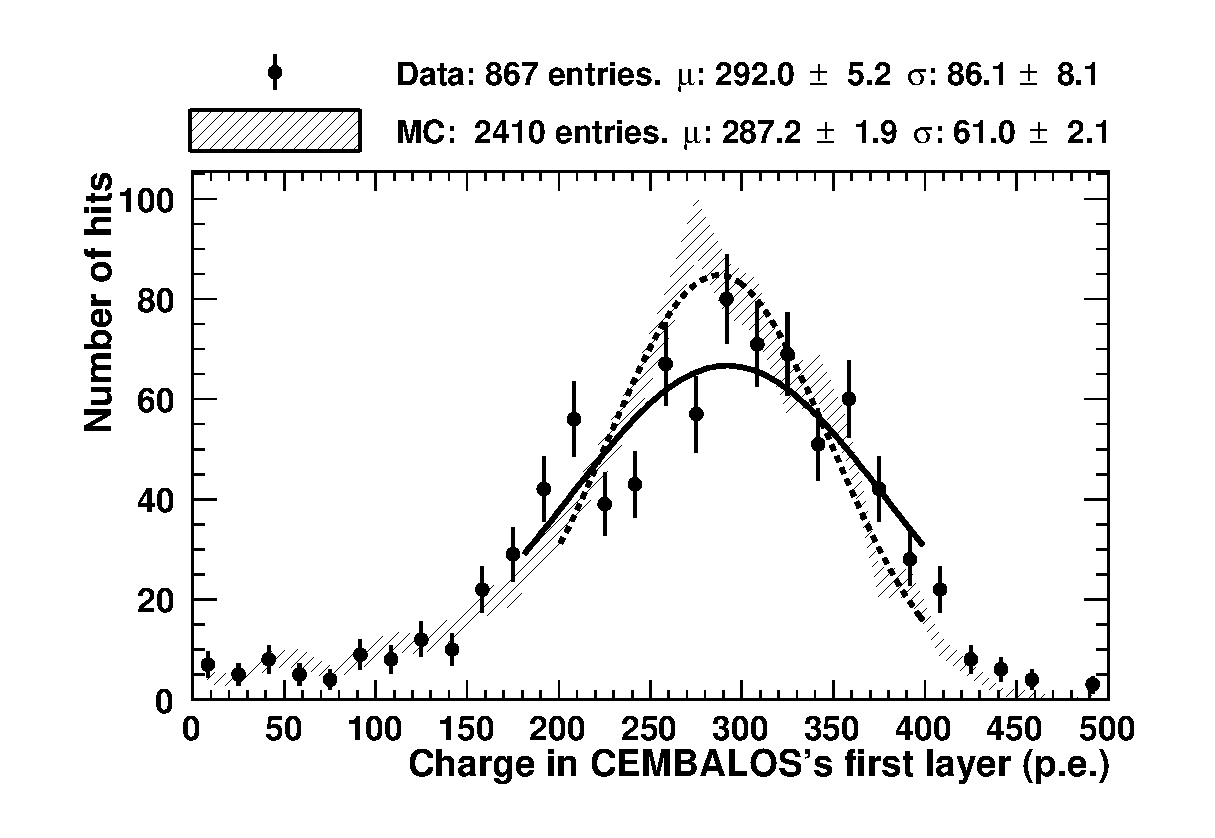
\includegraphics[width=86mm]{figures/proton_contained_1stlayer.eps}
 \caption{Charge distribution in the first layer of CEMBALOS for stopping protons in the 237.2 MeV$/c$ setting for data (circles) and MC (filled histogram). Only statistical uncertainties are plotted. The solid and dashed lines are Gaussian fits to data and MC respectively.}
 \label{fig:proton_sample}
\end{figure}

The accuracy of the charge simulation in the $>$50 p.e. region was estimated to be $\sim$20\% by comparing the Gaussian fits to the data and MC distributions shown in Fig \ref{fig:proton_sample}. The systematic uncertainty was propagated to the cross section measurement by applying a Gaussian smearing with a 20\% width to the charge deposition per event in 1000 toy MC experiments.

\subsubsection{\bf Hit inefficiency}
The hit reconstruction inefficiency in CEMBALOS was measured by counting how often a hit was missing in a reconstructed track. The tracks were required to have at least two hits in both the first and last two layers. Fig. \ref{fig:hit_ineff} shows the hit inefficiency, defined as the ratio of missing hits over the total number of hits expected, for data and MC in the 237.2 MeV$/c$ setting as a function of the CEMBALOS reconstructed polar angle. The hit inefficiency integrated over all angles is 1.33\% and 1.16\% for data and MC respectively.
\begin{figure}[ht]
 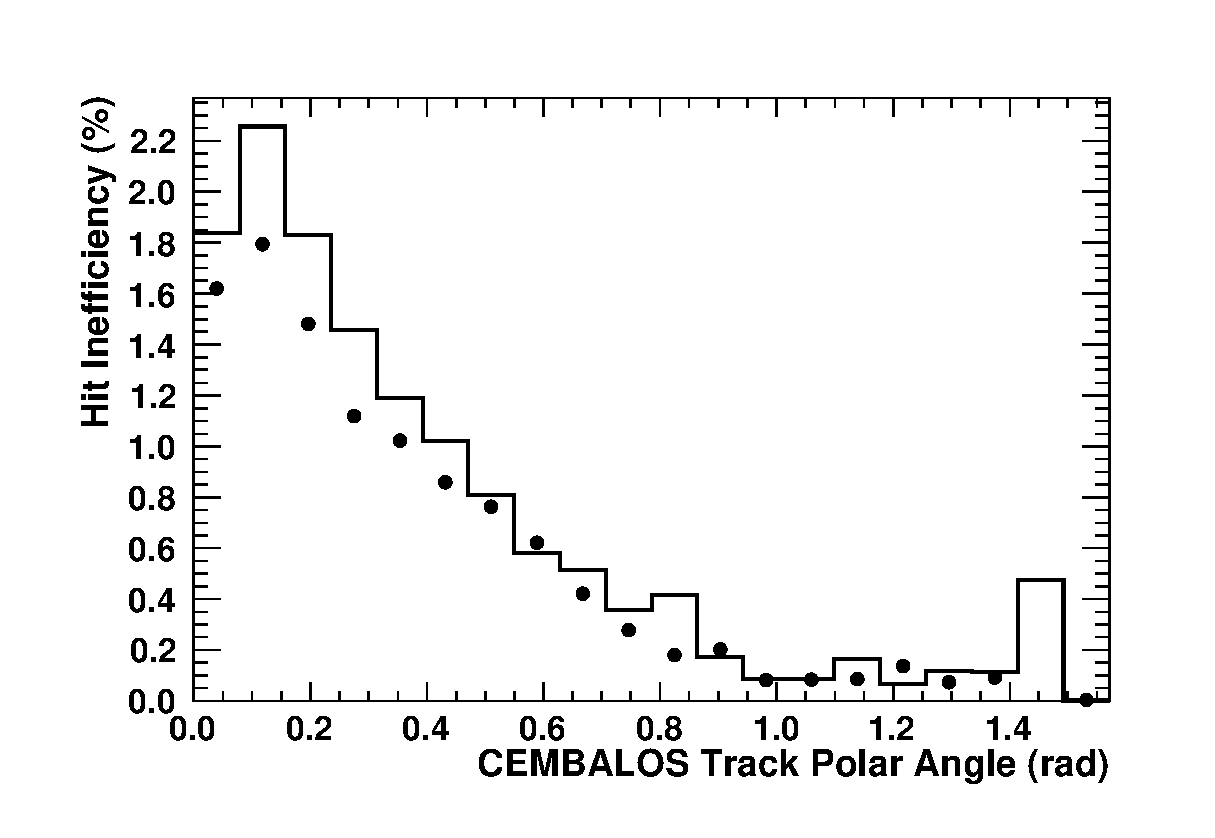
\includegraphics[width=86mm]{figures/cembalos_hit_ineff_237.eps}
 \caption{CEMBALOS hit inefficiency for data (circles) and MC (solid line) in the $p_\pi=$237.2 MeV$/c$ setting.}
 \label{fig:hit_ineff}
\end{figure}

The effect on the measured cross section is estimated by randomly deleting CEMBALOS hits in 1000 MC toy experiments with a probability given by the difference of the integrated hit inefficiencies for data and MC, affecting both the hit multiplicity and total charge deposited.

\subsection{Physics modeling systematics}\label{sec:physics_syst}
The kinematics of the outgoing $\pi^0$ from CX interactions is not well known. The only existing differential cross section measurement on light nuclei from Ashery \textit{et.al.} \cite{Ashery2} is of 265 MeV$/c$ $\pi^{+}$ on oxygen. A comparison of this data and predictions from the \textsc{Geant4} (v9.04.04) Bertini cascade model \cite{bertini}, the \textsc{Neut} (v5.3.5) cascade model \cite{NEUT} and the \textsc{Fluka} cascade model \cite{fluka1,fluka2} is shown on Fig. \ref{fig:pi0kinem}. The discrepancy among models is largest in the forward region, where CEMBALOS is most sensitive. In particular, the \textsc{Geant4} model used by our simulation shows the largest disagreement with data \cite{Ashery2}.

\begin{figure}[h]
 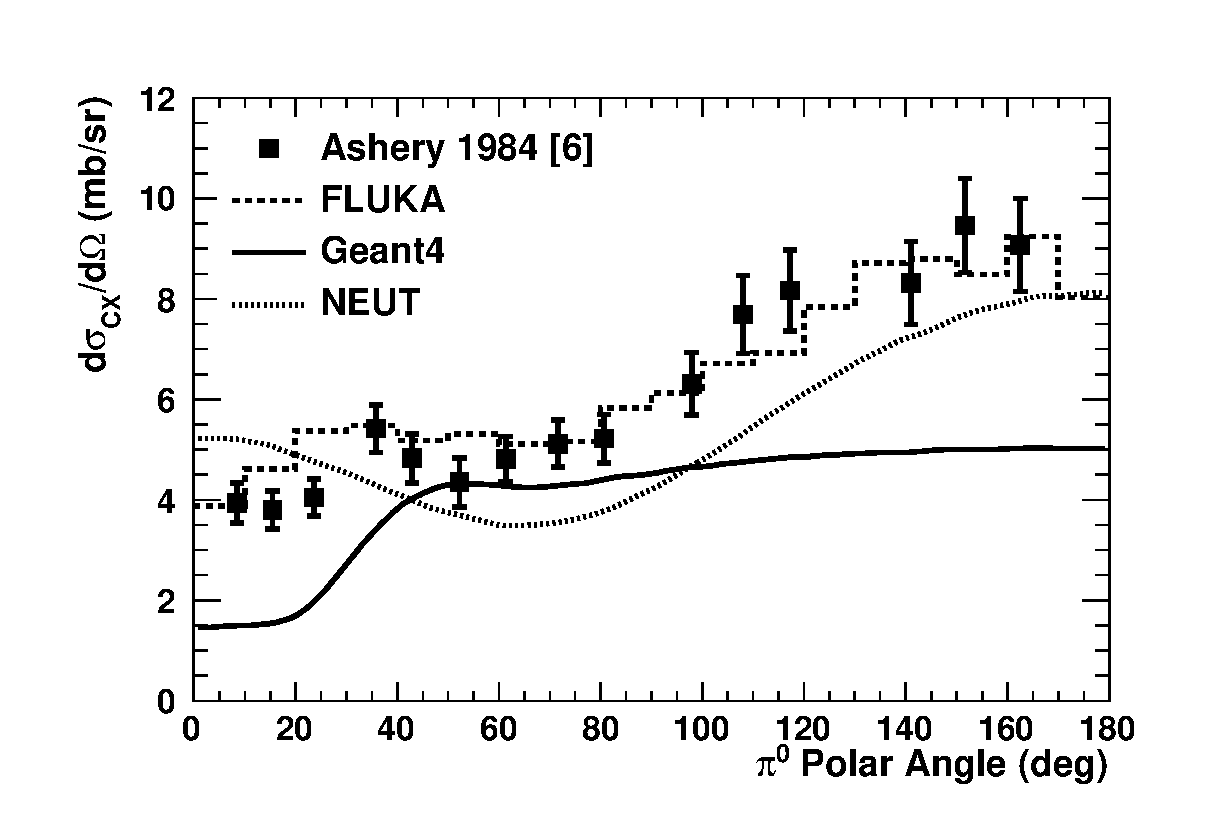
\includegraphics[width=86mm]{figures/dsigma_cx_o16_data_and_models.eps}
 \caption{$d\sigma_{\mathrm{CX}}/d\Omega$ as a function of the outgoing $\pi^0$ polar angle (in the lab frame) for 265 MeV$/c$ $\pi^{+}$ interacting on $^{16}$O, for \textsc{Fluka} (dashed line), \textsc{Geant4} (solid line) and \textsc{NEUT} (dotted line), along with data from \cite{Ashery2}.}
 \label{fig:pi0kinem}
\end{figure}

The modeling of the multiplicity and kinematics for nucleons ejected following an ABS or CX interaction show even larger discrepancies among models. The mechanisms for these processes are further complicated by the possibility of FSI of the nucleons before they exit the nucleus. Data on light nuclei that would help in the understanding and tuning of these processes is very scarce. \textsc{Neut} uses nucleon multiplicities published by \cite{Rowntree} of $\sigma_{\mathrm{ABS}}$ on N and Ar targets, but it is unclear what other models use. Despite the high purity of the events selected for this analysis, the effect of various models to our background prediction was investigated.

\subsubsection{\bf{Efficiency scheme}}
As was mentioned in Sec. \ref{section:calibration}, our simulation is based on the \textsc{Geant4} package which uses the Bertini cascade model for modeling pion inelastic interactions but also handles other complex aspects of the analysis such as the geometrical description of the detectors, simulates the electronics, etc. In order to investigate the effect of different models on the signal and background prediction without having to rewrite our simulation using each toolkit, we developed a scheme that replaces the detector simulation with a set of 2D selection and rejection efficiencies binned in $p$-$\theta$ bins of the outgoing particles described below. These were then applied to the predictions from \textsc{Neut} and \textsc{Fluka} obtained using thin target ($\sim1/X_{0}$) simulations.
\begin{enumerate}
\item{{\bf $\pi^0$ selection efficiency:} the probability of a true CX event passing the selection criteria as a function of the outgoing $\pi^0$ momentum and angle is defined as the ratio of the distributions before and after the selection is applied. This selection efficiency is shown in Fig. \ref{fig:pi0_selection} for the $p_{\pi}$ = 201.6 MeV$/c$ setting as an example.}

\begin{figure}[h]
 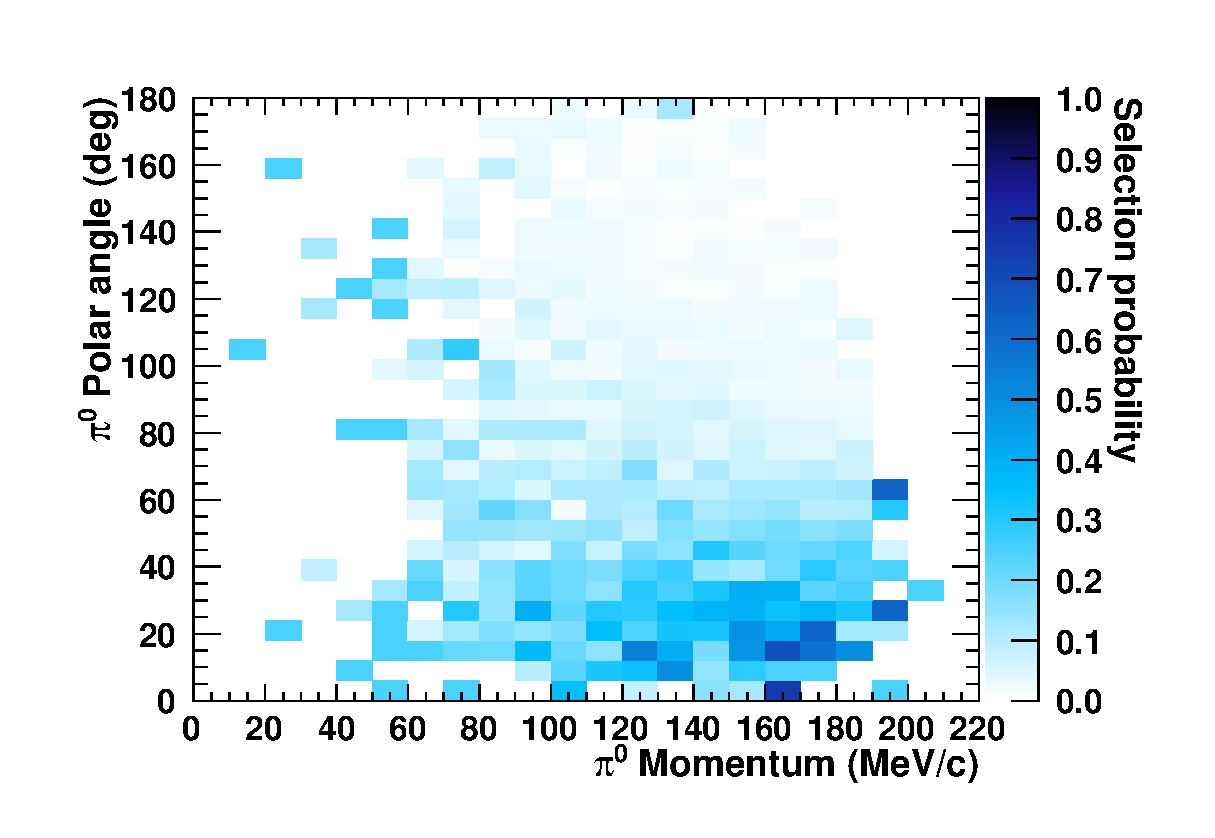
\includegraphics[width=86mm]{figures/Pi0SelectionEfficiency_200.eps}
 \caption{(Color online) Selection efficiency of true CX events as a function of the outgoing $\pi^{0}$ momentum and angle, for the $p_{\pi}$ = 201.6 MeV$/c$ setting.}
 \label{fig:pi0_selection}
\end{figure}

\item{{\bf Proton/neutron veto rejection:} the probability that an ejected proton or neutron will produce hits in the first two XY modules of CEMBALOS. Fig. \ref{fig:proton_rejection} shows the rejection efficiency for protons in the the 201.6 MeV$/c$ setting. The CEMBALOS forward acceptance ($<45^{\circ}$) can be clearly seen.}

\begin{figure}[h]
 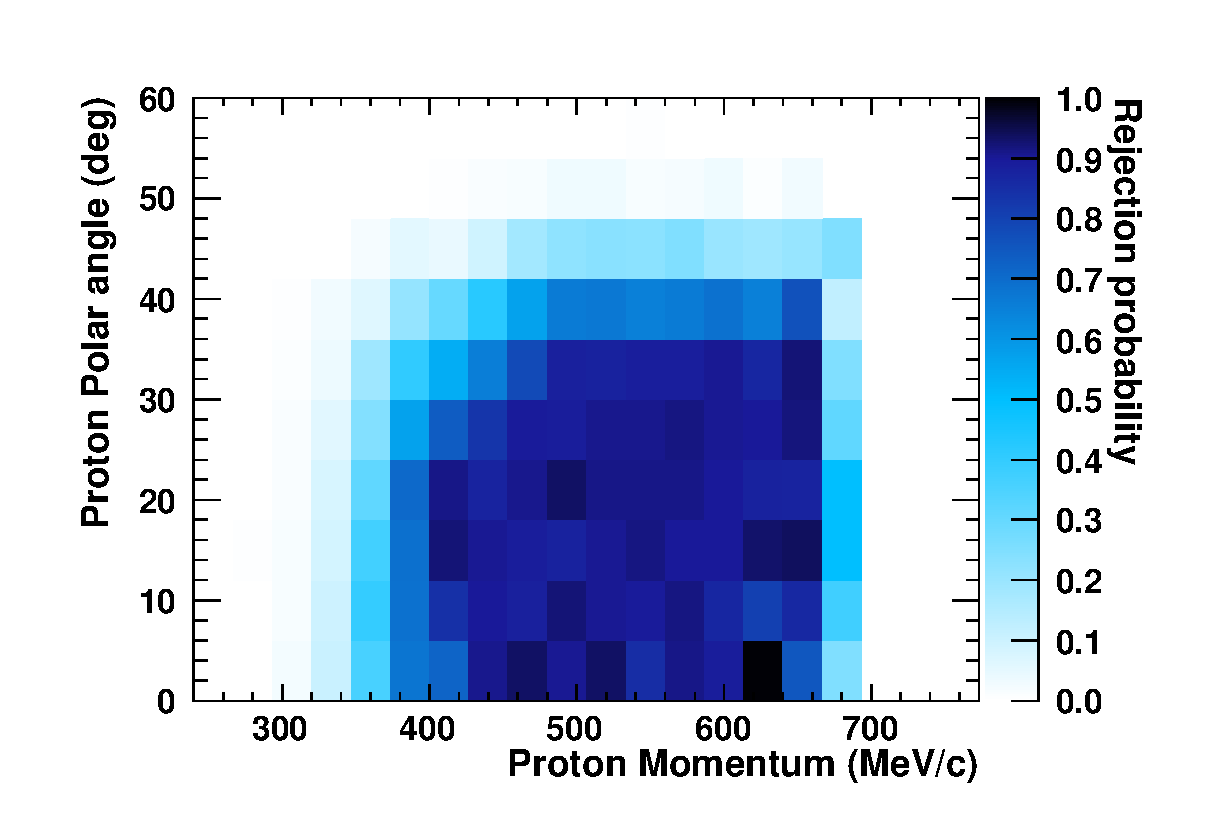
\includegraphics[width=86mm]{figures/ProtonRejectionEfficiency_200.eps}
 \caption{(Color online) Rejection probability of events where an eject protons from ABS or quasi-elastic scattering fails the veto rejection criteria, as a function of its outgoing  momentum and angle, for the $p_{\pi}$ = 201.6 MeV$/c$ setting.}
 \label{fig:proton_rejection}
\end{figure}

\item{{\bf Proton mis-reconstruction:} the probability of a proton being mis-reconstructed as a ``pion-like'' track in PIA$\nu$O thus causing the event to be rejected.}

\item{{\bf $\pi^{+}$ mis-reconstruction and veto:} the probability of an outgoing $\pi^{+}$ following a quasi-elastic scatter to be mis-reconstructed in PIA$\nu$O as a ``proton-like'' track and then producing hits in the first two XY modules of CEMBALOS.}

\item{{\bf Neutron selection efficiency:} the probability of a neutron from an ABS event passing the selection criteria.}
\end{enumerate}

In this scheme a true CX event would be categorized as a signal event if: the $\pi^{0}$ is selected, the ejected proton(s) is not mis-reconstructed as a ``pion-like'' track in PIA$\nu$O, and the ejected nucleons do not fire the veto rejection. On the other hand, an ABS or quasi-elastic scattering event would be categorized as a background event if: a neutron is selected, the outgoing $\pi^{+}$ is not mis-reconstructed as a proton, the ejected proton(s) is not mis-reconstructed in PIA$\nu$O as ``pion-like'', and the the ejected nucleons do not enable the veto rejection. 

The results of applying this scheme to model predictions from various models are summarized in Table \ref{tbl:eff_scheme_results} for each momentum setting. In addition to \textsc{Neut} and \textsc{Fluka}, the scheme was applied to the \textsc{Geant4} model prediction calculated from a thin target simulation (independent of the DUET simulation) as a means of validation of the procedure. The prediction of $N_{\mathrm{CX}}^{\mathrm{MC}}$ agrees with Table \ref{tbl:short_event_summary} within $\sim$3\%, while $N_{\mathrm{BG}}^{\mathrm{MC}}$ is underestimated as not all sources of background are included in the scheme. These are discussed in Sec. \ref{sec:background}.
\begin{table}[htbp]
\begin{center}
\begin{tabular}{c|c|c|c|c|c}
%\noalign{\hrule height 1pt}                                                                                                                       
\hline
$p_{\pi}$ [MeV$/c$] & Model & $\sigma_{CX}^{MC}$ [mb] &  $N_{\mathrm{CX}}^{\mathrm{MC}}$  &  $N_{\mathrm{BG}}^{\mathrm{MC}}$  &  $\sigma_{CX}$ [mb] \\ \hline
\multirow{4}{*}{201.6} %& DUET & 34.3 & 60.4 & 8.7 & 59.1 \\
& \textsc{Geant4} & 36.7 & 63.3 & 6.1 & 58.0 \\
& \textsc{Fluka} & 55.5 & 122.2 & 6.3 & 45.3 \\
& \textsc{Neut} & 50.5 & 83.0 & 4.5 & 61.8 \\ \hline

\multirow{4}{*}{216.6} %& DUET & 34.9 & 15.8 & 2.4 & 42.5 \\
& \textsc{Geant4} & 37.5 & 16.5 & 2.0 & 41.6 \\
& \textsc{Fluka} & 59.5 & 32.5 & 1.5 & 34.4  \\
& \textsc{Neut} & 55.7 & 24.2 & 1.5 & 43.5 \\ \hline

\multirow{4}{*}{237.2} %& DUET & 36.8 & 75.9 & 11.1 & 68.2 \\
& \textsc{Geant4} & 39.6 & 80.0 & 9.7 & 65.4 \\
& \textsc{Fluka} & 61.7 & 149.4 & 5.8 & 56.1 \\
& \textsc{Neut} & 57.5 & 111.7 & 6.1 & 69.8 \\ \hline

\multirow{4}{*}{265.5} %& DUET & 41.3 & 87.1 & 10.5 & 72.4 \\
& \textsc{Geant4} & 44.7 & 88.8 & 9.6 & 71.4 \\
& \textsc{Fluka} & 62.4 & 143.5 & 5.0 & 63.7 \\
& \textsc{Neut} & 57.9 & 129.4 & 6.9 & 64.8 \\ \hline

\multirow{4}{*}{295.1} %& DUET & 41.6 & 119.4 & 12.8 & 56.5 \\
& \textsc{Geant4} & 45.1 & 122.5 & 12.7 & 55.1 \\
& \textsc{Fluka} & 58.5 & 176.2 & 5.6 & 52.0 \\
& \textsc{Neut} & 58.3 & 170.3 & 8.4 & 52.7 \\ \hline
%\noalign{\hrule height 1pt}
\end{tabular}
\caption{Predicted $N_{\mathrm{CX}}^{\mathrm{MC}}$, $N_{\mathrm{BG}}^{\mathrm{MC}}$ and extracted CX cross section $\sigma_{\mathrm{CX}}$ obtained from applying the efficiency scheme to \textsc{Geant4}, \textsc{Fluka} and \textsc{Neut} model predictions. See text for discussion.}
\label{tbl:eff_scheme_results}
\end{center}
\end{table}

The differences in the extracted cross section among models range from 21.9\% at $p_{\pi}$ = 201.6 MeV$/c$ to 5.7\% at $p_{\pi}$ = 295.1 MeV$/c$, with \textsc{Fluka} and \textsc{Geant4} being the extreme case scenarios. This is consistent with the model comparison from Fig. \ref{fig:pi0kinem}. Considering the good agreement between \textsc{Fluka} and the external data in Fig. \ref{fig:pi0kinem}, the results from applying the efficiency scheme to \textsc{Fluka}, with the $N_{\mathrm{BG}}^{\mathrm{MC}}$ prediction scaled up to increase the additional backgrounds not included in the scheme, were chosen as our nominal result.

\subsubsection{\bf{$\pi^{0}$ kinematics reweighting}}
True CX events where reweighted following the discrepancy between \cite{Ashery2} and the \textsc{Fluka} model prediction as a function of the $\pi^{0}$ angle. The weights ranged from 0.7 to 1.3, while the average weight applied was 0.9. The effect on $\sigma_{\mathrm{CX}}$ ranged  from 6.1\% to 10.6\%, representing the largest systematic uncertainty for this analysis.

\subsubsection{\bf Other backgrounds}\label{sec:background}
The uncertainty from additional contributions to the number of predicted background events were estimated in three different categories, as described in the following text.

{ \it Nuclear de-excitation $\gamma$-rays:} inelastic interactions can leave the nucleus in an excited state. Low-energy ($<25$ MeV$/c$) $\gamma$-rays can be emitted as the nucleus returns to its ground state. If these photons interact in CEMBALOS they can fake a signal event. While these processes are believed to be well modeled by our simulation, we assign a conservative 100\% error on the number of background events from this process.\\

{ \it Multiple interactions: } it is possible for the initial $\pi^{+}$ to be scattered (both elastically or quasi-elastically) before it undergoes a CX interaction. The CX interaction can take place inside the PIA$\nu$O FV ($\sim$58\%), outside the FV but still in a scintillating fiber ($\sim$37\%), or somewhere in the aluminum support structure and/or dark boxes of PIA$\nu$O or CEMBALOS ($\sim$5\%). The uncertainty of the number of events of this type of background event is estimated from the uncertainty on elastic and CX interactions on carbon and aluminum from previous experiments.\\

{ \it $\pi^{+}$ decay products: } a $\pi^{+}$ that scatters in PIA$\nu$O and produces a fake ``proton-like'' track can then stop and decay around or inside CEMBALOS, possibly circumventing the veto rejection. The decay products can then deposit enough energy in CEMBALOS to produce a fake signal event. A conservative 100\% uncertainty is assigned to these events, which amount to $\sim$1\% of the selected events. %Fig. \ref{fig:ev_disp_decay} shows an example of these type of events

%\begin{figure}[ht]
%    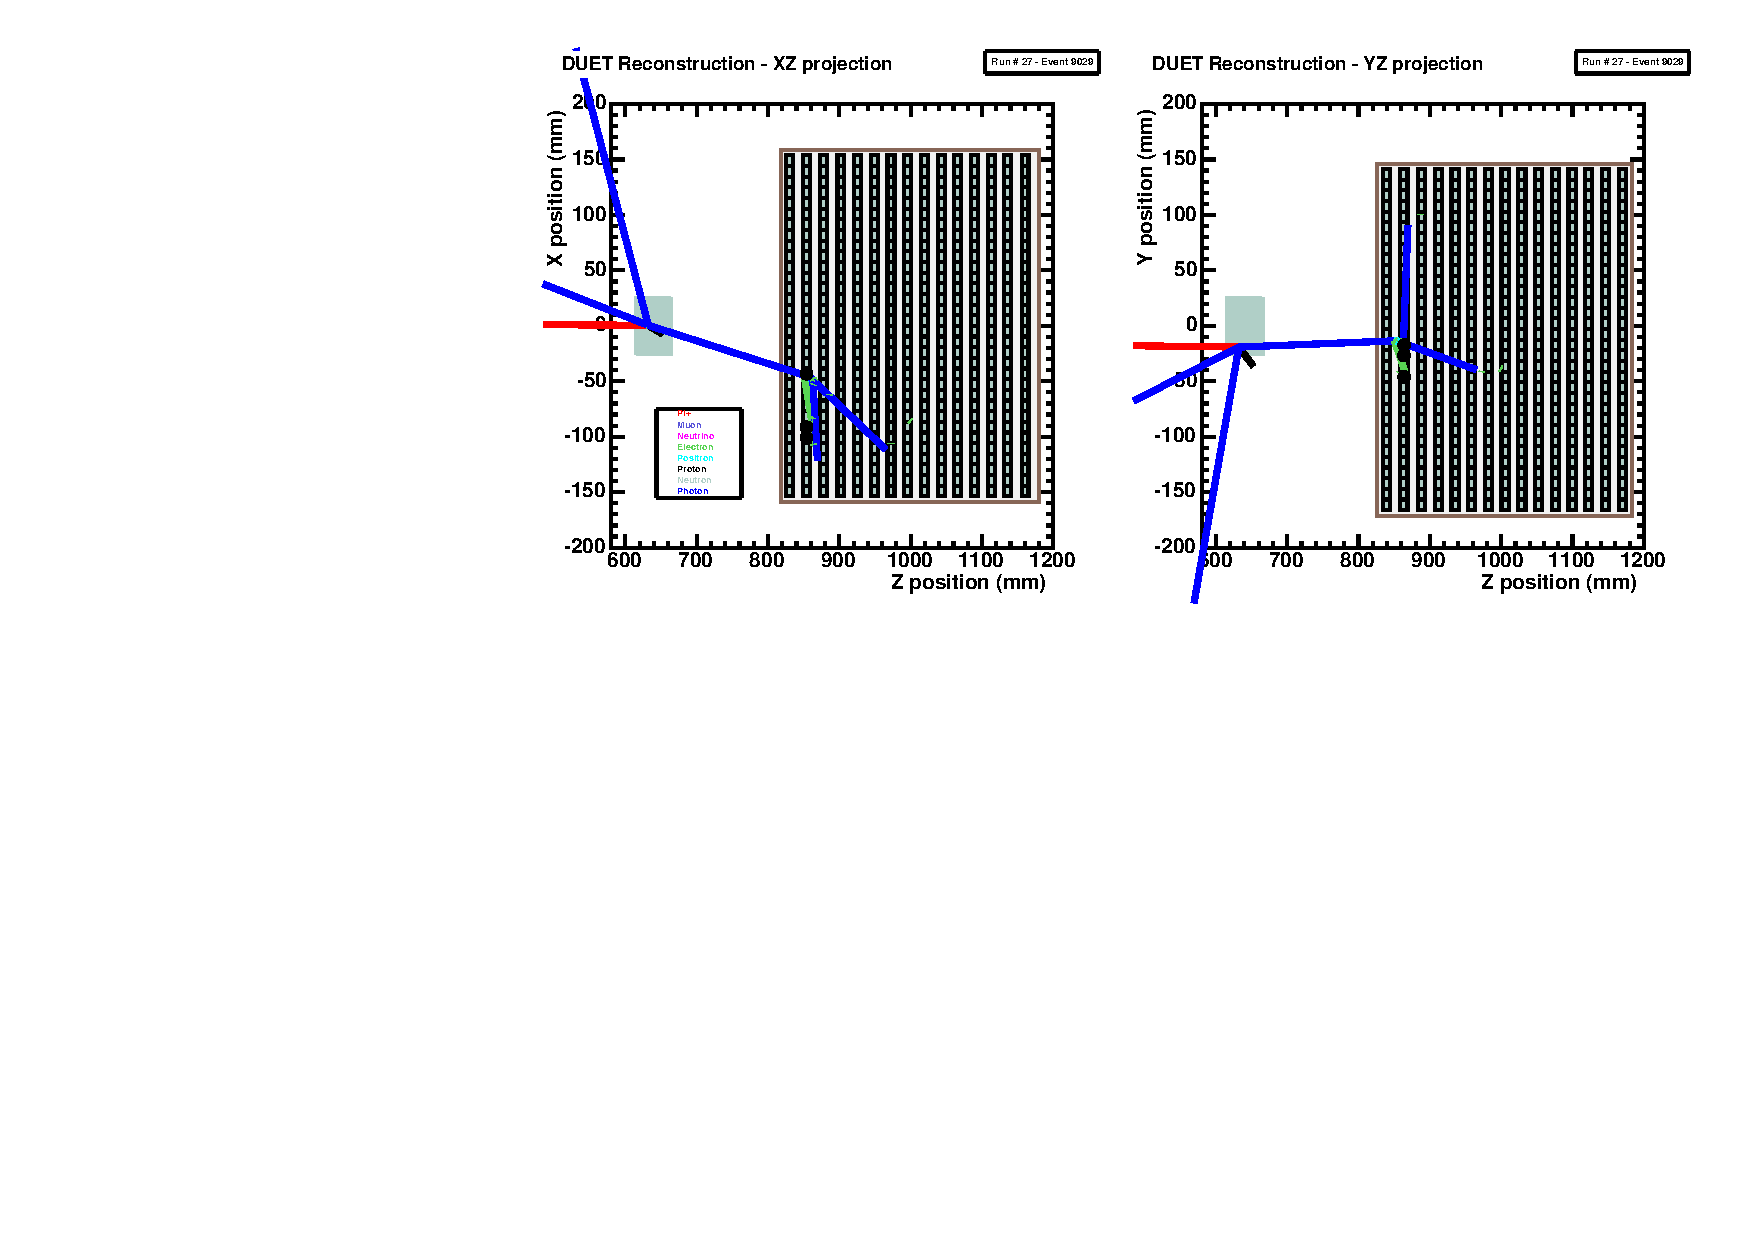
\includegraphics[width=90mm]{figures/ev_display_27_9029_intr4_ntag267.pdf}
%    \caption{Example of a CX event ($p_\pi=$237.2 MeV$/c$). A $\pi^+$ (red) undergoes CX in PIA$\nu$O resulting in a $\pi^0$ decay to two photons (blue). A forward-going photon is identified in CEMBALOS as it showers and hits are recorded in the scintillating material.}
%   \label{fig:ev_disp_decay}
%   \end{figure}

%\subsection{Summary of uncertainties}